\documentclass[12pt,aspectratio=169]{beamer}
\usetheme{metropolis}
\setbeamersize{text margin left=.5cm,text margin right=.5cm}
\usepackage[lf]{carlito}
\usepackage{tikz}
\usepackage{mathpazo}
\usepackage{xcolor,colortbl}
\usepackage{hyperref}
\usepackage{siunitx}
\setlength{\itemsep}{0pt}
\setlength{\parskip}{0pt}
\renewcommand{\baselinestretch}{1}

\sisetup{
  inter-unit-product=\cdot,
  per-mode=symbol
}
\tikzset{
  >=latex
}

\title{Topic 8: Mechanical Waves \& Sound}
\subtitle{Advanced Placement Physics 1}
\author[TML]{Dr.\ Timothy Leung}
\institute{Olympiads School}
\date{Updated: \today}

\newcommand{\pic}[2]{\includegraphics[width=#1\textwidth]{#2}}
\newcommand{\eq}[2]{\vspace{#1}{\Large\begin{displaymath}#2\end{displaymath}}}


\begin{document}

\begin{frame}
  \titlepage
\end{frame}



\section{Properties}

\begin{frame}{Mechanical Waves}
  A \textbf{mechanical wave} is a traveling disturbance that transport energy
  through a medium
  \begin{itemize}
  \item When a disturbance (vibration) causes vibrations in its vicinity, a
    wave is created
  \item Does not transport matter
  \item Examples:
    \begin{itemize}
    \item Sound wave (medium: air, solids and liquids)
    \item Ocean wave (medium: water)
    \item Wave on a string (medium: string, rope)
    \end{itemize}
  \item In contrast, electromagnetic (''EM'') waves do not require a medium
  \end{itemize}
\end{frame}




\begin{frame}{Two Kinds of Waves}
  \begin{center}
    \pic{.6}{main-qimg}
  \end{center}
  \begin{enumerate}[a.]
  \item\textbf{Longitudinal wave}
    \begin{itemize}
    \item Vibration is parallel to the direction of the motion of the wave
    \item Example: sound waves
    \end{itemize}
  \item\textbf{Transverse wave}
    \begin{itemize}
    \item Vibrations occur right angles to the direction of the wave
    \item Example: electromagnetic waves
    \end{itemize}
  \end{enumerate}
\end{frame}





\begin{frame}{Physical Properties of a Wave}
  \begin{itemize}
  \item The \emph{highest} point of the wave is called a \textbf{crest} or
    \textbf{peak}, while
  \item The \emph{lowest} point in the wave is called a \textbf{trough}.
  \item The \textbf{wavelength} $\lambda$ is the shortest distance between two
    points in the medium that are in phase. The easiest way to measure
    wavelength is from crest to crest, or from trough to trough.
  \end{itemize}
\begin{center}
    \vspace{-.2in}
    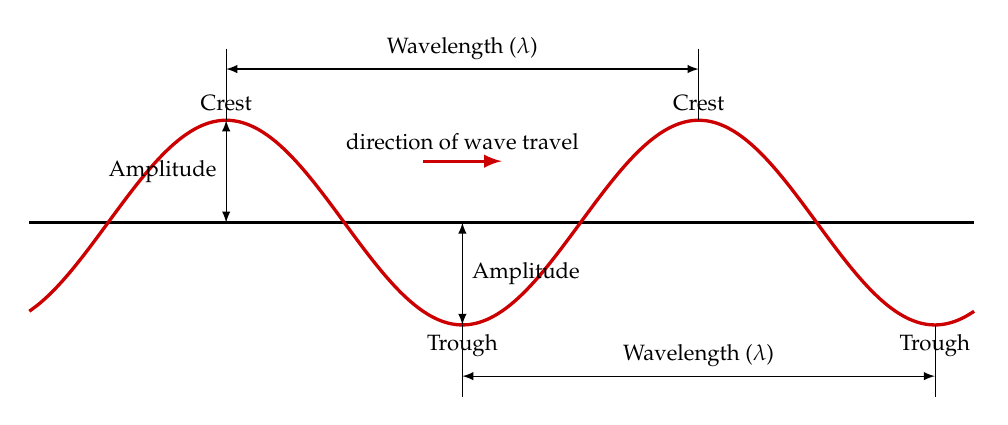
\begin{tikzpicture}[yscale=1.3]
      \draw[thick](0,0)--(12,0);
      \draw[very thick,red!80!black,smooth,samples=100,domain=0:12]
      plot({\x},{sin(60*(\x-1))});
      \draw[->,very thick,red!80!black](5,.6)--(6,.6)
      node[midway,above,black]{\footnotesize direction of wave travel};
      \draw[<->](2.5,1)--(2.5,0) node[midway,left] {\footnotesize Amplitude};
      \draw[<->](5.5,-1)--(5.5,0)node[midway,right]{\footnotesize Amplitude};
      \draw[<->](2.5,1.5)--(8.5,1.5)
      node[midway,above]{\footnotesize Wavelength ($\lambda$)};
      \draw[very thin](2.5,1.7)--(2.5,1) node[above]{\footnotesize Crest};
      \draw[very thin](8.5,1.7)--(8.5,1) node[above]{\footnotesize Crest};
      \draw[<->](5.5,-1.5)--(11.5,-1.5)
      node[midway,above]{\footnotesize Wavelength ($\lambda$)};
      \draw[very thin](5.5,-1.7)--(5.5,-1)   node[below]{\footnotesize Trough};
      \draw[very thin](11.5,-1.7)--(11.5,-1) node[below]{\footnotesize Trough};
    \end{tikzpicture}
\end{center}
\end{frame}


\section{Wave Equation}

\begin{frame}{The Wave Equation}
  The mechanical wave as we know it is the solution to a second-order partial
  differential equation: %\footnote{The equation is \emph{second order} because
  %it contains second derivatives, and \emph{partial} because it involves
  %partial derivatives with respect to both space $x$ and time $t$.}:
  
  \eq{-.2in}{
    \frac{\partial^2 u}{\partial t^2} = v^2\frac{\partial^2 u}{\partial x^2}
  }

  subject to initial condition.
\end{frame}



\begin{frame}{Equation of a Traveling Wave}
  One solution to the wave equation is a \textbf{harmonic wave} that can be
  described as a sinusoidal function that oscillates in both space $x$ and time
  $t$:
  
  \eq{-.2in}{
    \boxed{u(x,t)=A\sin(kx-\omega t)}
  }
  \begin{center}
    \begin{tabular}{l|c|c}
      \rowcolor{pink}
      \textbf{Quantity} & \textbf{Symbol} & \textbf{SI Unit} \\ \hline
      Displacement of the medium  & $u$ & \si\metre \\
      Amplitude of the wave       & $A$ & \si\metre \\
      Wave number                 & $k$ & \si{\per\metre} \\
      Distance from the source    & $x$ & \si\metre \\
      Time                        & $t$ & \si\second \\
      Angular frequency           & $\omega$ & \si{\per\second}
    \end{tabular}
  \end{center}
\end{frame}




\begin{frame}{Equation of a Traveling Wave}
  \eq{-.1in}{
    \boxed{u(x,t)=A\sin(kx-\omega t)}
  }

  \vspace{-.1in}The angular frequency (angular velocity) is related to the
  frequency $f$ and period $T$ of the wave by:

  \eq{-.35in}{
    \omega=\frac{2\pi}T=2\pi f
  }

  The \textbf{wave number} $k$ can be thought of as a the ``spatial frequency''
  of the wave, and is related to the wavelength $\lambda$ by:
  
  \eq{-.2in}{
    k=\frac{2\pi}\lambda
  }
\end{frame}



\begin{frame}{Universal Wave Equation}
  The \textbf{universal wave equation} relates the speed of a mechanical wave
  to its wavelength, period and frequency of the disturbance:

  \eq{-.15in}{
    \boxed{v = f\lambda =\frac{\lambda}T}
  }
  \begin{center}
    \begin{tabular}{l|c|c}
      \rowcolor{pink}
      \textbf{Quantity} & \textbf{Symbol} & \textbf{SI Unit} \\ \hline
      Speed         & $v$       & \si{\metre\per\second} \\
      Frequency     & $f$       & \si\hertz \\
      Wavelength    & $\lambda$ & \si\metre \\
      Period        & $T$       & \si\metre 
    \end{tabular}
  \end{center}
  The universal wave equation applies to \emph{all} waves. %For sound waves,
  %$v=v_\text{sound}$; for electromagnetic waves $v=c$.
\end{frame}




\begin{frame}{Speed of a Wave}
  Using the universal wave equation, we fin that the speed of a wave can be
  related to the wave number and angular frequency by:

  \eq{-.2in}{
    v=\frac{\lambda}T=\frac{2\pi/k}{2\pi/\omega}=\frac{\omega}k
  }
\end{frame}



\begin{frame}{Why Sine and Cosines}
  French mathematician Joseph Fourier showed that \emph{all} periodic functions
  can be represented as an infinite series of $\sin$ and/or $\cos$ functions:

  \vspace{-.35in}{\Large
    \begin{align*}
      f(x)=&a_1\sin(x)+a_2\sin(2x)+a_3\sin(3x)+\ldots+\\
      &b_1\cos(x)+b_2\cos(2x)+b_3\cos(3x)+\ldots\\
      =&\sum_{n=1}^{\infty}a_n\sin(nx)+\sum_{n=1}^{\infty}b_n\cos(nx)
    \end{align*}
  }

  The sum is called the \textbf{Fourier series}. Depending on the shape of the
  wave, some coefficients $a_n$ and $b_n$ are zeros. This part is particularly
  important to sound waves.
\end{frame}



\begin{frame}{Making a Square Wave with Sine Waves}
  \begin{columns}    
    \column{.6\textwidth}
    \centering
    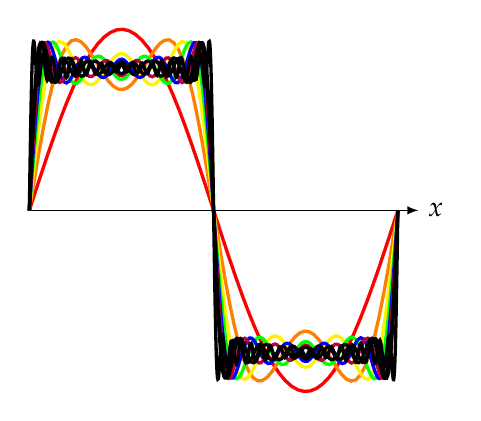
\begin{tikzpicture}[xscale=.013,yscale=2.3]
      \draw[->](0,0)--(380,0) node[right]{$x$};
      \uncover<1>{
        \draw[samples=60,domain=0:360,red,very thick]plot({\x},{sin(\x)});
      }
      \uncover<2>{
        \draw[samples=80,domain=0:360,orange,very thick]
        plot({\x},{sin(\x)+1/3*sin(3*\x)});
      }
      \uncover<3>{
        \draw[samples=100,domain=0:360,yellow,very thick]
        plot({\x},{sin(\x)+1/3*sin(3*\x)+1/5*sin(5*\x)});
      }
      \uncover<4>{
        \draw[smooth,samples=140,domain=0:360,green,very thick]
        plot({\x},{sin(\x)+1/3*sin(3*\x)+1/5*sin(5*\x)+1/7*sin(7*\x)});
      }
      \uncover<5>{
        \draw[smooth,samples=160,domain=0:360,blue,very thick]
        plot({\x},
        {sin(\x)+1/3*sin(3*\x)+1/5*sin(5*\x)+1/7*sin(7*\x)+1/9*sin(9*\x)});
      }
      \uncover<6>{
        \draw[smooth,samples=160,domain=0:360,purple,very thick]
        plot({\x},
        {sin(\x)+1/3*sin(3*\x)+1/5*sin(5*\x)+1/7*sin(7*\x)+1/9*sin(9*\x)+
          1/11*sin(11*\x)});
      }
      \uncover<7>{
        \draw[smooth,samples=200,domain=0:360,very thick]
        plot({\x},
        {sin(\x)+1/3*sin(3*\x)+1/5*sin(5*\x)+1/7*sin(7*\x)+1/9*sin(9*\x)+
          1/11*sin(11*\x)+
          1/13*sin(13*\x)});
      }
      \uncover<8>{
        \draw[smooth,samples=200,domain=0:360,very thick]
        plot({\x},
        {sin(\x)+1/3*sin(3*\x)+1/5*sin(5*\x)+1/7*sin(7*\x)+1/9*sin(9*\x)+
          1/11*sin(11*\x)+
          1/13*sin(13*\x)+
          1/15*sin(15*\x)});
      }
      \uncover<9>{
        \draw[smooth,samples=350,domain=0:360,very thick]
        plot({\x},
        {sin(\x)+1/3*sin(3*\x)+1/5*sin(5*\x)+1/7*sin(7*\x)+1/9*sin(9*\x)+
          1/11*sin(11*\x)+ 1/13*sin(13*\x)+ 1/15*sin(15*\x)+ 1/17*sin(17*\x)+
          1/19*sin(19*\x)+
          1/21*sin(21*\x)+ 1/23*sin(23*\x)+ 1/25*sin(25*\x)+ 1/27*sin(27*\x)+
          1/29*sin(29*\x)+
          1/31*sin(31*\x)+ 1/33*sin(33*\x)+ 1/35*sin(35*\x)+ 1/17*sin(37*\x)+
          1/39*sin(39*\x)});
      }
    \end{tikzpicture}

    \column{.35\textwidth}
    \uncover<1->{
      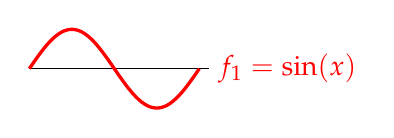
\begin{tikzpicture}[xscale=.006,yscale=.5]
        \draw(0,0)--(380,0) node[right]{\color{red}$f_1=\sin(x)$};
        \draw[samples=60,domain=0:360,red,very thick] plot({\x},{sin(\x)});
      \end{tikzpicture}
    }
    \uncover<2->{
      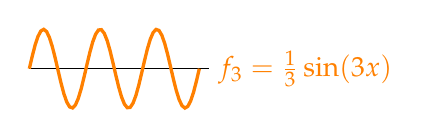
\begin{tikzpicture}[xscale=.006,yscale=.5]
        \draw(0,0)--(380,0) node[right]
             {\color{orange}$f_3=\frac13\sin(3x)$};
        \draw[samples=60,domain=0:360,orange,very thick] plot({\x},{sin(3*\x)});
      \end{tikzpicture}
    }
    \uncover<3->{
      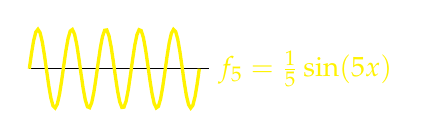
\begin{tikzpicture}[xscale=.006,yscale=.5]
        \draw(0,0)--(380,0) node[right]
             {\color{yellow}$f_5=\frac15\sin(5x)$};
        \draw[samples=80,domain=0:360,yellow,very thick] plot({\x},{sin(5*\x)});
      \end{tikzpicture}
    }
    \uncover<4->{
      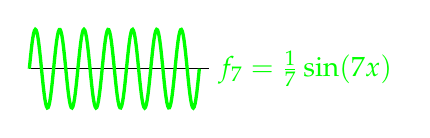
\begin{tikzpicture}[xscale=.006,yscale=.5]
        \draw(0,0)--(380,0) node[right]
             {\color{green}$f_7=\frac17\sin(7x)$};
        \draw[samples=200,domain=0:360,green,very thick] plot({\x},{sin(7*\x)});
      \end{tikzpicture}
    }
    \uncover<5->{
      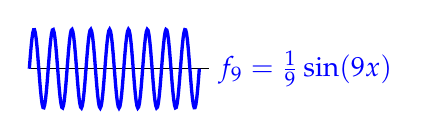
\begin{tikzpicture}[xscale=.006,yscale=.5]
        \draw(0,0)--(380,0) node[right]
             {\color{blue}$f_9=\frac19\sin(9x)$};
        \draw[samples=200,domain=0:360,blue,very thick] plot({\x},{sin(9*\x)});
      \end{tikzpicture}
    }
  \end{columns}
\end{frame}


\begin{frame}{Fourier Series and Harmonic Frequencies}
  \begin{center}
    \vspace{-.3in}
    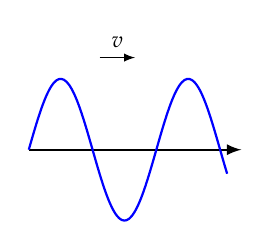
\begin{tikzpicture}[scale=.9]
      \draw[->,thick](0,0) --(3,0);
      \draw[->](1,1.3)--(1.5,1.3) node[midway,above]{\footnotesize $v$};
      \draw[thick,blue,smooth,samples=80,domain=0:2.8] plot({\x},{sin(200*\x)});
    \end{tikzpicture}
    \hspace{.15in}
    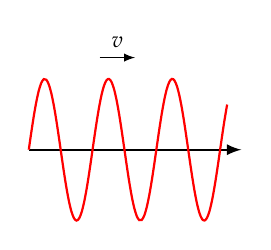
\begin{tikzpicture}[scale=.9]
      \draw[->,thick](0,0) --(3,0);
      \draw[->](1,1.3)--(1.5,1.3) node[midway,above]{\footnotesize $v$};
      \draw[thick,red,smooth,samples=80,domain=0:2.8] plot({\x},{sin(400*\x)});
    \end{tikzpicture}
    \hspace{.15in}
    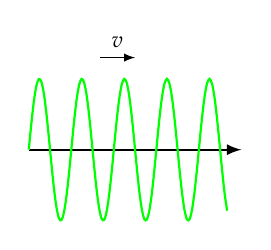
\begin{tikzpicture}[scale=.9]
      \draw[->,thick](0,0) --(3,0);
      \draw[->](1,1.3)--(1.5,1.3) node[midway,above]{\footnotesize $v$};
      \draw[thick,green,smooth,samples=80,domain=0:2.8]
      plot({\x},{sin(600*\x)});
    \end{tikzpicture}
  \end{center}

  \vspace{-.2in}
  \begin{itemize}
  \item The first wave (longest wavelength and lowest frequency) is called the
    \textbf{fundamental frequency}, or \textbf{first harmonic}
  \item The second term has half the wavelength and twice the frequency. It's
    called the \textbf{second harmonic}, the \textbf{first overtone}
  \item Also, third, fourth, fifth\ldots harmonics
  \end{itemize}
\end{frame}



\begin{frame}{Harmonic Frequencies}
    Every whole-number multiples of the fundamental frequency $f_1$ is its
    harmonic frequency, i.e.\ the $n$-th harmonic is:

    \eq{-.25in}{
      \boxed{f_n=nf_1}\quad n=1,2,3,\ldots
    }
    For sound waves, when a musical instrument produces a sound that has, the
    frequency that is ``heard'' is the fundamental frequency
\end{frame}


\section{Wave Speed}

\begin{frame}{Frequency and Speed of A Wave}
  Frequency ($f$):
  \begin{itemize}
  \item The number of complete wavelengths that pass a point in a given amount
    of time
  \item Same as the frequency of the disturbance that generated the wave
  \item\textbf{Does not depend on the medium}, only the source that produced
    the wave
  \end{itemize}

  \vspace{.2in}Wave speed ($v$)
  \begin{itemize}
  \item The speed at which the wave fronts are moving
  \item \textbf{Depends only on the medium}, not the source disturbance that
    produced the wave
  \item Within the same medium, waves of different wavelengths can travel
    at different speeds
  \end{itemize}
\end{frame}



\begin{frame}{Speed of Sound in a Gas}
  The speed of an \textbf{acoustic wave} (sound wave) in a gas is given by:
  
  \eq{-.2in}{
    \boxed{v_s=\sqrt{\frac{\gamma RT}M}}
  }
  \begin{center}
    \begin{tabular}{l|c|c}
      \rowcolor{pink}
      \textbf{Quantity} & \textbf{Symbol} & \textbf{SI Unit} \\ \hline
      Wave speed             & $v_s$    & \si{\metre\per\second}\\
      Temperature            & $T$      & \si{\kelvin}\\
      Universal gas constant & $R$      & \si{\joule/mol.\kelvin}\\
      Molar mass             & $M$      & \si{\kilo\gram/mol}\\
      Adiabatic constant     & $\gamma$ & (no units)
    \end{tabular}
  \end{center}
  For diatomic gases such as air $\gamma=1.4$, and
  $M=\SI{29e-3}{\kilo\gram/mol}$. For air near room temperature, the equation
  can be simplified to: $\boxed{v_s=331+0.59T_C}$ where $T_c$ is the
  temperature in \emph{degrees celsius}.
\end{frame}



\begin{frame}{Speed of Sound in Solids and Liquids}
  \begin{columns}
    \column{.6\textwidth}
    Speed of sound in a liquid depends on the ``bulk modulus'' $K$ and density
    $\rho$ of the liquid:
      
    \eq{-.2in}{
      v=\sqrt{\frac{K}\rho}
    }
   
    Speed of sound in a solid depends on the ``Young's modulus'' $E$ of the
    solid and density $\rho$

    \eq{-.2in}{
      v=\sqrt{\frac{E}\rho}
    }

    \vspace{-.1in}In general, sound travels fastest in solids, then liquids,
    then gasses.
    
    \column{.4\textwidth}
    \begin{tabular}{l|c}
      \rowcolor{blue!30}
      \textbf{Material} & \textbf{Speed} (\si{\metre\per\second}) \\
      \rowcolor{pink!70}
      \multicolumn2c{Gases (\SI0\celsius, \SI{101}{\kilo\pascal})} \\
      Carbon dioxide & 259 \\
      Oxygen         & 316 \\
      Air            & 331 \\
      Helium         & 965 \\
      \rowcolor{pink!70}
      \multicolumn2c{Liquids (\SI{20}\celsius)} \\
      Ethanol        & 1162 \\
      Fresh water    & 1482 \\
      Seawater       & 1440-1500 \\
      \rowcolor{pink!70}
      \multicolumn2c{Solids} \\
      Copper         & 5010 \\
      Glass          & 5640 \\
      Steel          & 5960
    \end{tabular}
  \end{columns}
\end{frame}



\begin{frame}{Wave on a String}
  The speed of a traveling wave on a stretched string is determined by:
  
  \eq{-.2in}{
    \boxed{v=\sqrt{\frac{F_T}{\mu}}}
    \quad\text{\normalsize where}\quad
    \boxed{\mu=\frac{m}L}
  }
  \begin{center}
    \begin{tabular}{l|c|c}
      \rowcolor{pink}
      \textbf{Quantity} & \textbf{Symbol} & \textbf{SI Unit} \\ \hline
      Wave speed           & $v$   & \si{\metre\per\second} \\
      Tension              & $F_T$ & \si\newton \\
      Linear mass density  & $\mu$ & \si{\kilo\gram\per\metre} \\
      Mass of the string   & $m$   & \si{\kilo\gram} \\
      Length of the string & $L$   & \si\metre
    \end{tabular}
  \end{center}
\end{frame}



\begin{frame}{Speed of an Surface Ocean Wave}
  The speed of a surface wave in deep ocean is given by:
  
  \eq{-.2in}{
    \boxed{v=\sqrt{\frac{\lambda g}{2\pi}}}
  }
  \begin{center}
    \begin{tabular}{l|c|c}
      \rowcolor{pink}
      \textbf{Quantity} & \textbf{Symbol} & \textbf{SI Unit} \\ \hline
      Wave speed           & $v$       & \si{\metre\per\second} \\
      Wavelength           & $\lambda$ & \si\metre \\
      Acceleration due to gravity & $g$ & \si{\metre\per\second\squared}
    \end{tabular}
  \end{center}
  In this case, in an ocean wave, the higher frequency (shorter wavelength)
  travel faster than the lower frequency waves (longer wavelength). This is
  called \textbf{dispersion}.
\end{frame}





\begin{frame}{Wave Simulation}
  A helpful simulation can be found on the PhET website at University of
  Colorado.
  \begin{center}
    \textbf{Click for external link:}\\
    \href{https://phet.colorado.edu/sims/html/wave-on-a-string/latest/wave-on-a-string_en.html}
         {wave on a string simulation}
  \end{center}
\end{frame}



\begin{frame}{Power Transmitted by a Harmonic Wave}
  The total power $\overline{P}$ transmitted by a harmonic wave on a string is
  given by:

  \eq{-.2in}{
    \boxed{\overline{P}=\frac12\mu\omega^2A^2v}
  }
  \begin{center}
    \begin{tabular}{l|c|c}
      \rowcolor{pink}
      \textbf{Quantity} & \textbf{Symbol} & \textbf{SI Unit} \\ \hline
      Averge power        & $\bar{P}$ & \si\watt \\
      Linear mass density & $\mu$     & \si{\kilo\gram\per\metre}\\
      Angular frequency   & $\omega$  & \si{rad\per\second}\\
      Wave amplitude      & $A$       & \si\metre \\
      Wave speed          & $v$       & \si{\metre\per\second}
    \end{tabular}
  \end{center}  
\end{frame}



\begin{frame}{Intensity of a 3D Wave}
  For a three dimension waves (e.g.\ sound waves, ripple in pond) where the
  wave front expands as the wave travels, it makes more sense to describe the
  power transmitted by its \textbf{intensity} $I$:

  \eq{-.25in}{
    \boxed{I=\frac{\overline{P}}S}
  }

  For a spherical wave (e.g.\ sound emitted from a stationary source), the area
  that the wavefront passes through is $S=4\pi r^2$, where $r$ is the distance
  from the source.
\end{frame}



\begin{frame}{The Decibel}
  The \textbf{decibel} is defined as by the intensity of sound $I$ compared to
  the \textbf{threshold of hearing} $I_o$ (defined as
  \SI{1e-12}{\watt\per\metre\squared}):
  
  \eq{-.2in}{
    \boxed{\beta=10\log_{10}\left[\frac{I}{I_0}\right]}
  }
  \begin{center}
    \begin{tabular}{l|c|c}
      \rowcolor{pink}
      \textbf{Quantity} & \textbf{Symbol} & \textbf{SI Unit} \\ \hline
      Decibel              & $\beta$ & \si{dB}\\
      Sound intensity      & $I$     & \si{\watt\per\metre\squared}\\
      Threshold of hearing & $I_0$   & \si{\watt\per\metre\squared}
    \end{tabular}
  \end{center}  
  
  \begin{itemize}
  \item The threshold of hearing is \SI0{dB}, while the
    \textbf{threshold of pain} is \SI{120}{dB}.
  \item Humans perceive a doubling of loudness when intensity is increases by a
    factor of 10 (an increase of \SI{10}{dB})
  \end{itemize}
\end{frame}



\begin{frame}{Mach Number}
  When dealing with sound waves, it is often useful to express speed in terms
  of its ratio to the speed of sound, called the \textbf{mach number}:
  
  \eq{-.2in}{
    \boxed{M=\frac{v}{v_s}}
  }
  \begin{center}
    \begin{tabular}{l|c|c}
      \rowcolor{pink}
      \textbf{Quantity} & \textbf{Symbol} & \textbf{SI Unit} \\ \hline
      Mach number          & $M$   & (no units) \\
      Speed of the object  & $v$   & \si{\metre\per\second}\\
      Local speed of sound & $v_s$ & \si{\metre\per\second}
    \end{tabular}
  \end{center}
  \begin{itemize}
  \item Speeds lower than $M<1$ is called \emph{subsonic}
  \item Speeds higher than $M>1$ is called \emph{supersonic}
  \end{itemize}
\end{frame}



\begin{frame}{Sound from a Stationary Source}
  When a sound is emitted from a stationary point source, the sound wave moves
  radially outward from the origin:
  \begin{center}
    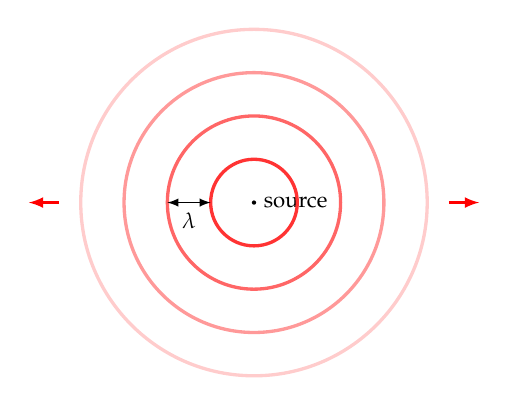
\begin{tikzpicture}[scale=.55]
      \fill[black](0,0) circle(.05) node[right]{\footnotesize source};
      \begin{scope}[very thick]
        \uncover<2->{ \draw[red!80](0,0) circle(1); }
        \uncover<3->{ \draw[red!60](0,0) circle(2); }
        \uncover<4->{ \draw[red!40](0,0) circle(3); }
        \uncover<5->{ \draw[red!20](0,0) circle(4); }
      \end{scope}
      \uncover<5->{
        \draw[<->](-1,0)--(-2,0) node[midway,below]{\footnotesize $\lambda$};
        \draw[thick,->,red](4.5,0)--(5.2,0);
        \draw[thick,->,red](-4.5,0)--(-5.2,0);
      }
    \end{tikzpicture}
    \begin{itemize}
    \item Sound intensity (amplitude) drops farther away from the source
    \item All points hear the same wavelength (and frequency) of sound
    \end{itemize}
  \end{center}
\end{frame}



\subsection{Doppler Effect \& Shock Waves}

\begin{frame}{Sound from a Moving Source}
  When sound is emitted from a \emph{moving} source, the diagram looks
  different. In this case, the sound source is moving to the right, from $1$ to
  $4$:
  \vspace{.2in}
  \begin{columns}
    \column{.3\textwidth}
    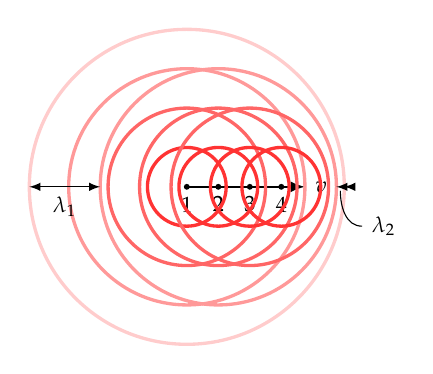
\begin{tikzpicture}[scale=.5]
      \fill ( 0,0) circle(.075) node[below]{\footnotesize 1};
      \uncover<2->{ \fill (.8,0) circle(.075) node[below]{\footnotesize 2}; }
      \uncover<3->{ \fill(1.6,0) circle(.075) node[below]{\footnotesize 3}; }
      \uncover<4->{ \fill(2.4,0) circle(.075) node[below]{\footnotesize 4}; }
      \draw[thick,->](0,0)--(3,0) node[right]{\footnotesize $v$};
      \begin{scope}[very thick]
        \uncover<2>{
          \draw[red!80](0,0) circle(1);
        }
        \uncover<3>{
          \draw[red!60](0,0) circle(2);
          \draw[red!80](.8,0)circle(1);
        }
        \uncover<4>{
          \draw[red!40]  (0,0) circle(3);
          \draw[red!60] (.8,0) circle(2);
          \draw[red!80](1.6,0) circle(1);
        }
        \uncover<5>{
          \draw[red!20](  0,0) circle(4);
          \draw[red!40]( .8,0) circle(3);
          \draw[red!60](1.6,0) circle(2);
          \draw[red!80](2.4,0) circle(1);
        }
      \end{scope}
      \uncover<5->{
        \draw[<->](-4,0)--(-2.2,0)
        node[midway,below]{\footnotesize $\lambda_1$};
        \draw[<->](4,0)--(3.8,0);
        \node (a) at (5,-1) {\footnotesize $\lambda_2$};
        \draw(3.9,-.1) to[out=270,in=180] (a);
      }
    \end{tikzpicture}
      
    \column{.7\textwidth}
    \uncover<5>{
      \begin{itemize}
      \item When the source is moving \emph{toward you}, the wavelength
        $\lambda_2$ decreases, and the apparent frequency increases.
      \item When the source is moving \emph{away from you}, the wavelength
        $\lambda_1$ increases, and the aparent frequency decreases.
      \end{itemize}

      \vspace{.2in}This is called the \textbf{Doppler effect}.
    }
  \end{columns}
\end{frame}



\begin{frame}{Doppler Effect}
  We all experience Doppler effect every time an ambulance speeds by us with
  its sirens on.
  \begin{center}
    \pic{.6}{toronto-ambulance}
  \end{center}
  When it is moving toward us, the pitch of the siren is high, but the moment
  it passes us, the pitch decreases.
\end{frame}



\begin{frame}{Doppler Effect}
  When a wave source is moving at a speed $v_\text{src}$ and an observing is
  moving at observer $v_\text{ob}$, the perceived frequency is shifted:

  \eq{-.2in}{
    \boxed{f'=\frac{v_s\pm v_\text{ob}}{v_s\mp v_\text{src}}f}
  }
  \begin{center}
    \begin{tabular}{l|c|c}
      \rowcolor{pink}
      \textbf{Quantity} & \textbf{Symbol} & \textbf{SI Unit} \\ \hline
      Apparent frequency  & $f'$   & \si\hertz \\
      Actual frequency    & $f$    & \si\hertz \\
      Speed of sound      & $v_s$ & \si{\metre\per\second}\\
      Speed of source & $v_\text{src}$ & \si{\metre\per\second}\\
      Speed of observer & $v_\text{ob}$ & \si{\metre\per\second}
    \end{tabular}
  \end{center}
  The $+$ sign is used if the source and observer are approaching each other,
  and $-$ is when they are receding
\end{frame}




\begin{frame}{Sound Source at Sonic Speed}
  Doppler effect is even more interesting is when sound source is moving at the
  speed of sound ($M=1$):
  \vspace{.2in}
  \begin{columns}
    \column{.32\textwidth}
    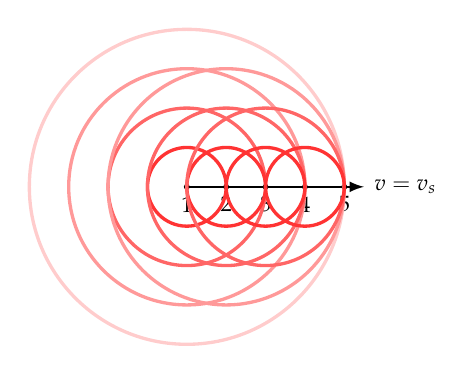
\begin{tikzpicture}[scale=.5]
      \draw[->,thick](0,0)--(4.5,0) node[right]{\footnotesize $v=v_s$};
      \fill(0,0) circle(.075) node[below]{\footnotesize $1$};
      \uncover<2->{ \fill(1,0) circle(.075) node[below]{\footnotesize $2$}; }
      \uncover<3->{ \fill(2,0) circle(.075) node[below]{\footnotesize $3$}; }
      \uncover<4->{ \fill(3,0) circle(.075) node[below]{\footnotesize $4$}; }
      \uncover<5->{ \fill(4,0) circle(.075) node[below]{\footnotesize $5$}; }

      \begin{scope}[very thick]
        \uncover<2>{
          \draw[red!80](0,0) circle(1);
        }
        \uncover<3>{
          \draw[red!60](0,0) circle(2);
          \draw[red!80](1,0)circle(1);
        }
        \uncover<4>{
          \draw[red!40](0,0) circle(3);
          \draw[red!60](1,0) circle(2);
          \draw[red!80](2,0) circle(1);
        }
        \uncover<5>{
          \draw[red!20](0,0) circle(4);
          \draw[red!40](1,0) circle(3);
          \draw[red!60](2,0) circle(2);
          \draw[red!80](3,0) circle(1);
        } 
      \end{scope}
    \end{tikzpicture}
      
    \column{.68\textwidth}
    \uncover<5>{
      \begin{itemize}
      \item The wavefronts (crests) from all the waves are bunched up just in
        front of the source
      \item Since sound wave is a pressure wave, right in front of the sound
        source, there is a large change in pressure (called a shock wave)
      \item When the shock passes an observer, an loud bang can be heard (aka
        \textbf{sonic boom})
    }
    \end{itemize}
  \end{columns}
\end{frame}



\begin{frame}{Sound from a Supersonic Source}
  When sound source is moving at $M>1$, it out runs the sound that it makes:
  \begin{columns}
    \column{.47\textwidth}
    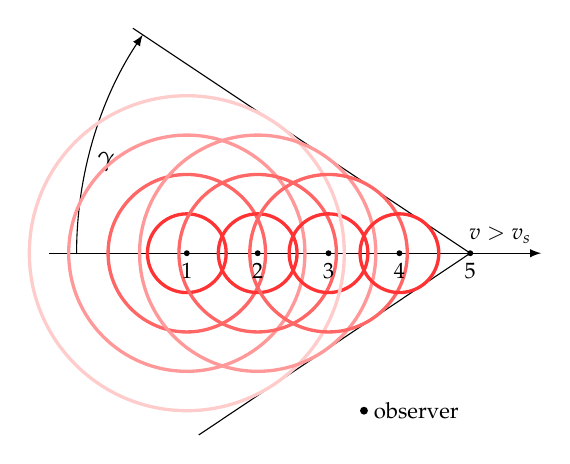
\begin{tikzpicture}[scale=.5]
      
      \draw[->](-3.5,0)--(9,0) node[above left]{\footnotesize $v>v_s$};
      \uncover<5>{
        \draw[rotate around={213.8:(7.2,0)}](7.2,0)--(15.5,0);
        \draw[rotate around={146.3:(7.2,0)}](7.2,0)--(17.5,0);
        \draw[->](-2.8,0) arc(180:146.3:10) node[pos=.4,right]{$\gamma$};
        \fill[black](4.5,-4) circle(.1) node[right]{\footnotesize observer};
      }
      \begin{scope}[very thick]
        \uncover<2>{
          \draw[red!80](0,0) circle(1);
        }
        \uncover<3>{
          \draw[red!60](0,0) circle(2);
          \draw[red!80](1.8,0)circle(1);
        }
        \uncover<4>{
          \draw[red!40](0,0) circle(3);
          \draw[red!60](1.8,0) circle(2);
          \draw[red!80](3.6,0) circle(1);
        }
        \uncover<5>{
          \draw[red!20](0,0) circle(4);
          \draw[red!40](1.8,0) circle(3);
          \draw[red!60](3.6,0) circle(2);
          \draw[red!80](5.4,0) circle(1);
        } 
      \end{scope}
      \fill(0,0) circle(.075) node[below]{\footnotesize $1$};
      \uncover<2->{ \fill(1.8,0) circle(.075) node[below]{\footnotesize $2$}; }
      \uncover<3->{ \fill(3.6,0) circle(.075) node[below]{\footnotesize $3$}; }
      \uncover<4->{ \fill(5.4,0) circle(.075) node[below]{\footnotesize $4$}; }
      \uncover<5->{ \fill(7.2,0) circle(.075) node[below]{\footnotesize $5$}; }
    \end{tikzpicture}
      
    \column{.53\textwidth}
    \uncover<5>{
      An \emph{oblique shock} is formed at an angle (called the
      \textbf{Mach angle}) given by:
      
      \eq{-.1in}{
        \gamma=\sin^{-1}\left(\frac1M\right)
      }

      An observer does not hear the sound source until it has gone past!
    }
  \end{columns}
\end{frame}



\begin{frame}{Bullet in Supersonic Flight}
  Generating a shock doesn't require an actual sound source. Any object
  moving through air creates a pressure disturbance. Below is a NATO bullet in
  supersonic flight:
  \begin{center}
    \pic{.35}{bullet2}
  \end{center}
  The flow around this bullet is taken inside a \emph{shock tube} that
  generates a short burst of supersonic flow. A high-speed camera is used to
  take the photo.
\end{frame}



\begin{frame}{Duck in Water}
  A similar shock behavior is observed when the duck swims in water, because
  the duck swims faster than the speed of the water wave, it also creates a
  cone shape.
  \begin{center}
    \pic{.5}{duck}
  \end{center}

\end{frame}



\section{Reflection and Transmission}

\begin{frame}{Reflection of a Wave at a Boundary}
  \begin{columns}
    \column{.5\textwidth}
    When a wave on a string reflects at a boundary, how the reflected wave looks
    depends on the type of boundary
    \begin{itemize}
    \item At a \emph{fixed end} (left):
      \begin{itemize}
      \item the reflected wave is \emph{inverted}
      \item i.e.\ a phase shift of $\pi$
      \item i.e.\ a crest becomes a trough
      \end{itemize}
    \item At a \emph{free end} (right)
      \begin{itemize}
      \item the reflected wave is upright
      \item No phase shifts
      \end{itemize}
    \end{itemize}
    
    \column{.5\textwidth}
    \pic1{22}
  \end{columns}
\end{frame}


\begin{frame}{Transmission of Waves: Fast to Slow Medium}
  \begin{columns}
    \column{.6\textwidth}
    \begin{itemize}
    \item Reflected wave:
      \begin{itemize}
      \item Inverted, like a fixed end
      \item Same frequency and wavelength as the incoming wave
      \item The amplitude is decreased because energy is split between the
        reflected and transmitted waves
      \end{itemize}
    \item Transmitted wave:
      \begin{itemize}
      \item Upright
      \item Same frequency as incoming wave, but has a shorter wavelength
        because the wave slowed down
      \end{itemize}
    \end{itemize}
    
    \column{.4\textwidth}
    \pic1{23}
  \end{columns}
\end{frame}


\begin{frame}{Transmission of Waves: Slow to Fast Medium}
  \begin{columns}
    \column{.6\textwidth}
    \begin{itemize}
    \item Reflected wave:
      \begin{itemize}
      \item Upright, like a free end
      \item Same frequency and wavelength as the incoming wave
      \item The amplitude is decreased because energy is split between the
        reflected and transmitted waves
      \end{itemize}
    \item Transmitted wave:
      \begin{itemize}
      \item Upright
      \item Same frequency as incoming wave, but has a longer wavelength because
        the wave sped up
      \end{itemize}
    \end{itemize}
    
    \column{.4\textwidth}
    \pic1{24}
  \end{columns}
  Note that the transmitted wave is \emph{always} upright.
\end{frame}



\section[Interference]{Wave Interference}

\begin{frame}{Superposition of Waves}
  \begin{center}
    \pic{.6}{omkAt}
  \end{center}
  \begin{itemize}
  \item\textbf{Principle of Superposition:} When multiple waves pass through
    the same point, the resultant wave is the \emph{sum} of the waves
    \begin{itemize}
    \item A fancy way of saying that waves add together
    \end{itemize}
  \item The consequence of the principle of superposition is
    \textbf{interference of waves}. There are two kinds of interference:
    \begin{itemize}
    \item\textbf{Constructive interference:} Two wave fronts (crests) passing
      through creates a wave front with greater amplitude
    \item\textbf{Destructive interference:} A crest and trough will cancel
      each other
    \end{itemize}
  \end{itemize}
\end{frame}



\begin{frame}{Superposition of Waves}
  \begin{columns}
    \column{.6\textwidth}
    \textbf{Constructive interference}: In-phase wave fronts sum together
    \begin{itemize}
    \item In this example, two identical pulses move towards each other
    \item Their crests pass through A at the same time
    \item The amplitude at A when the waves pass through is higher 
    \end{itemize}
    
    \column{.4\textwidth}
    \pic1{constructive}
  \end{columns}
\end{frame}



\begin{frame}{Superposition of Waves}
  \begin{columns}
    \column{.65\textwidth}
    \textbf{Destructive interference}: Out-of-phase wave fronts shows the
    difference of the wave fronts
    \begin{itemize}
    \item Two pulses move towards each other, one a crest, the other a trough
    \item They both pass through A at the same time
    \item Two waves cancel each other at A
    \end{itemize}
        
    \column{.35\textwidth}
    \pic1{destructive}
  \end{columns}
\end{frame}


\begin{frame}{Beat Frequency}
  When waves (e.g.\ sound waves) of two different frequencies are added
  together, there is both constructive and destructive interference because of
  the principle of superposition
  \begin{itemize}
  \item Plotting two functions representing two waves with equal magnitude
    and wave speed $v_s$: $\color{blue}{y=\sin(x)}$
    \uncover<2->{and $\color{red}{y=\sin(1.1x)}$}
  \end{itemize}
  \begin{center}
    \vspace{-.1in}
    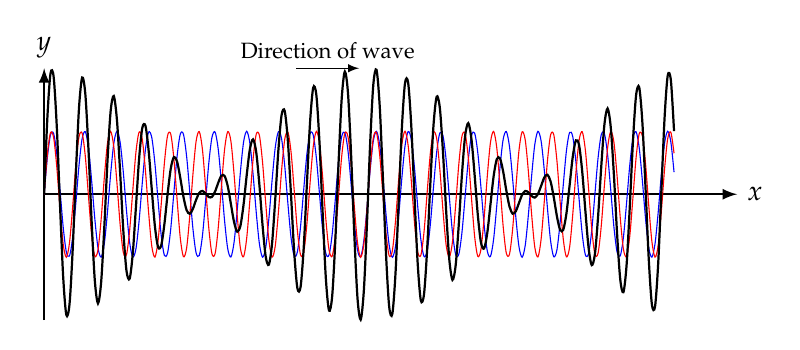
\begin{tikzpicture}[scale=.8]
      \draw[->,thick](0,0) --(11,0) node[right] {$x$};
      \draw[->,thick](0,-2)-- (0,2) node[above] {$y$};
      \draw[->](4,2)--(5,2) node[midway,above]{\footnotesize Direction of wave};
      \uncover<1,3->{
        \draw[blue,smooth,samples=200,domain=0:10] plot({\x},{sin(700*\x)});
      }
      \uncover<2->{
        \draw[smooth,samples=200,domain=0:10,red] plot({\x},{sin(770*\x)});
      }
      \uncover<4>{
        \draw[smooth,samples=200,domain=0:10,thick]
        plot({\x},{sin(700*\x)+sin(770*\x)});
      }
    \end{tikzpicture}
  \end{center}
  \uncover<4->{
    \vspace{-.1in}
    \begin{itemize}
    \item The thick black line is the sum: $y=\sin(x) + \sin(1.1x)$
    \end{itemize}
  }
\end{frame}



\begin{frame}{Beats}
  The \textbf{beat frequency} is the absolute difference of the frequencies of
  the two component waves:

  \eq{-.2in}{
    \boxed{f_\text{beat}=|f_1-f_2|}
  }
  \begin{center}
    \begin{tabular}{l|c|l}
      \rowcolor{pink}
      \textbf{Quantity} & \textbf{Symbol} & \textbf{SI Unit} \\ \hline
      Beat frequency     & $f_\text{beat}$    & \si\hertz \\
      Frequency of 1st component wave & $f_1$ & \si\hertz \\
      Frequency of 2nd component wave & $f_2$ & \si\hertz
    \end{tabular}
  \end{center}
  For sound waves, they sound like a pulsating ``whoomf''. Musicians often use
  the beat frequencies to determine whether someone is play in tune or out of
  tune.
\end{frame}



\begin{frame}{Standing Waves}
  \begin{center}
    \pic{.6}{standing-wave-3}
  \end{center}
  If two waves of the same frequency meet up under the right conditions, they
  may appear to be ``standing still''. This is called a standing wave
  \begin{itemize}
  \item Node: A point that never moves
  \item Anti-node: A point which moves/vibrates maximally
  \end{itemize}
\end{frame}



\begin{frame}{Standing Waves}
  Two identical waves (blue \& yellow) move in opposite directions in the
  same medium. At some moment in time, they are out of phase, resulting in
  destructive interference (green):
  \begin{center}
    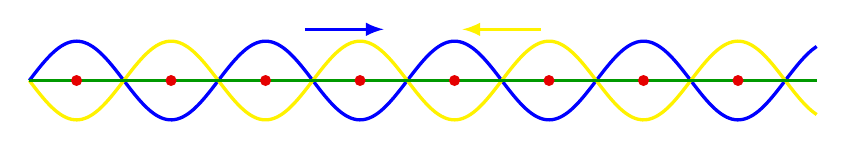
\begin{tikzpicture}
      \draw[very thick,->,blue](3.5,.65)--(4.5,.65);
      \draw[very thick,->,yellow](6.5,.65)--(5.5,.65);
      \draw[smooth,samples=150,domain=0:10,blue,very thick]
      plot({\x},{.5*sin(150*\x)});
      \draw[smooth,samples=150,domain=0:10,yellow,very thick]
      plot({\x},{-.5*sin(150*\x)});
      \draw[very thick,green!60!black](0,0)--(10,0);
      \foreach \x in {0.6,1.8,...,10} \fill[red!90!black](\x,0) circle(.07);
    \end{tikzpicture}
  \end{center}
  A quarter of a wavelength later, the 2 waves are in phase (constructive
  interference):
  \begin{center}
    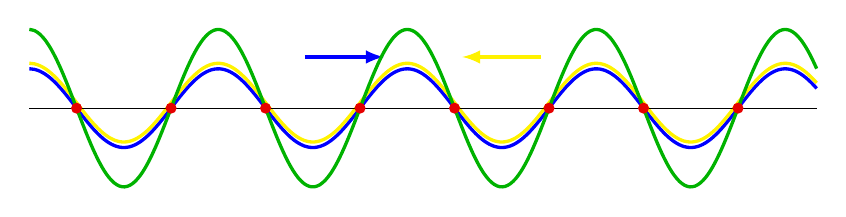
\begin{tikzpicture}
      \draw[very thick,->,blue](3.5,.65)--(4.5,.65);
      \draw[very thick,->,yellow](6.5,.65)--(5.5,.65);
      \draw[smooth,samples=150,domain=0:10,blue,very thick]
      plot({\x},{.5*sin(150*\x+90)});
      \draw[smooth,samples=150,domain=0:10,yellow,very thick]
      plot({\x},{-.5*sin(150*\x-90)+0.07});
      \draw[smooth,samples=150,domain=0:10,green!70!black,very thick]
      plot({\x},{sin(150*\x+90)});
      \draw(0,0)--(10,0);
      \foreach \x in {.6,1.8,...,10} \fill[red!90!black](\x,0) circle(.07);
    \end{tikzpicture}
  \end{center}
  But regardless of whether the wave is in phase, the red dots always have zero
  displacement. They are called \textbf{nodes}.
\end{frame}



\section{Standing Waves}

\begin{frame}{Standing Waves On a String}
  \begin{itemize}
  \item A ``vibrating'' string is actually a standing wave on a string
  \item Both ends of the string are nodes
  \item As the string vibrates, the air around it vibrates at the same frequency
  \item The vibration travels as a sound wave toward your ears
  \item Examples:
    \begin{itemize}
    \item Plucking a guitar or violin string
    \item Hitting a key on a piano/harpsichord
    \end{itemize}
  \end{itemize}
\end{frame}



\begin{frame}{Standing Waves On a String of Length $L$}
  \textbf{Resonance frequencies} are frequencies where a standing wave can be
  created. The first resonance (fundamental) frequency at occurs when
  $\lambda=2L$:
  \begin{center}
    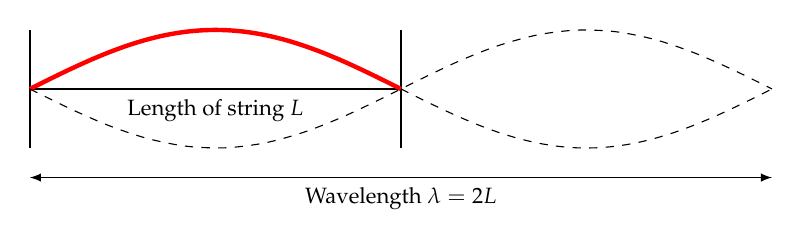
\begin{tikzpicture}[scale=1.5]
      \draw[thick](0,0) -- (pi,0)
      node[midway,below]{\footnotesize Length of string $L$};
      \draw[thick](0,-.5) --(0,.5);
      \draw[thick](pi,-.5)--(pi,.5);
      \draw[smooth,samples=20,domain=0:pi,red,ultra thick]
      plot({\x},{0.5*sin(180/pi*\x)});
      \draw[smooth,samples=20,domain=pi:2*pi,dashed]
      plot({\x},{0.5*sin(180/pi*\x)});
      \draw[smooth,samples=20,domain=0:2*pi,dashed]
      plot({\x},{-.5*sin(180/pi*\x)});
      \draw[<->](0,-.75)--(2*pi,-.75)
      node[midway,below]{\footnotesize Wavelength $\lambda=2L$};
    \end{tikzpicture}
  \end{center}
  
  \vspace{-.1in}The fundamental frequency is based on the speed of the
  traveling wave along the string $v_\text{str}$:

  \eq{-.3in}{
    \boxed{
      f_{r,1}
      =\frac{v_\text{str}}\lambda=\frac{v_\text{str}}{2L}}
  }
\end{frame}



\begin{frame}{Standing Waves On a String of Length $L$}
  A second resonance frequency occurs when $L=\lambda$:

  \vspace{-.2in}\begin{columns}
    \column{.45\textwidth}
    \centering
    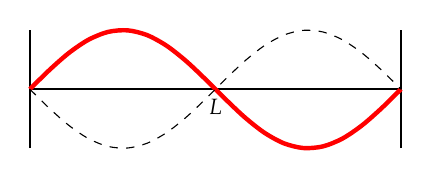
\begin{tikzpicture}[scale=1.5]
      \draw[thick](0,0)--(pi,0) node[midway,below]{\footnotesize $L$};
      \draw[thick](0,-.5)--(0,.5);
      \draw[thick](pi,-.5)--(pi,.5);
      \draw[smooth,samples=20,domain=0:pi,red,ultra thick]
      plot({\x},{.5*sin(360/pi*\x)});
      \draw[smooth,samples=20,domain=0:pi,dashed]
      plot({\x},{-.5*sin(360/pi*\x)});
    \end{tikzpicture}
    
    \column{.55\textwidth}
    
    \eq{-.01in}{
      f_{r,2}=
      \frac{v_\text{str}}\lambda=\frac{v_\text{str}}{L}=2f_{r,1}
    }
  \end{columns}

  And a third resonance frequency occurs at $\displaystyle L=\frac32\lambda$:

  \vspace{-.2in}
  \begin{columns}
    \column{.45\textwidth}
    \centering
    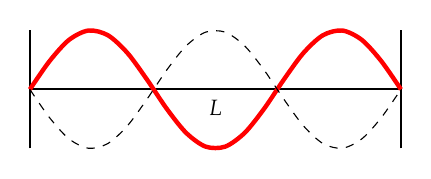
\begin{tikzpicture}[scale=1.5]
      \draw[thick](0,0)--(pi,0) node[midway,below]{\footnotesize $L$};
      \draw[thick](0,-.5)--(0,.5);
      \draw[thick](pi,-.5)--(pi,.5);
      \draw[smooth,samples=20,domain=0:pi,red,ultra thick]
      plot({\x},{.5*sin(540/pi*\x)});
      \draw[smooth,samples=20,domain=0:pi,dashed]
      plot({\x},{-.5*sin(540/pi*\x)});
    \end{tikzpicture}
    
    \column{.55\textwidth}
      
    \eq{-.01in}{
      f_{r,3}=\frac{3v_\text{str}}{2L}=3f_{r,1}
    }
  \end{columns}
\end{frame}



\begin{frame}{Standing Waves On a String of Length $L$}
  The $n$-th resonance frequency of a wave on string is given by:

  \eq{-.15in}{
    \boxed{f_n=nf_1}\quad
    \text{\normalsize where}\quad
    \boxed{f_1=\frac{v_\text{str}}{2L}}
  }
  \begin{itemize}
  \item $n$ is a whole-number multiple
  \item This equation is \emph{identical} to the equation for harmonic
    frequencies, meaning that on a string, every harmonic is a resonance
    frequency
  \item A vibrating string is said to have a ``full set of harmonics''
  \end{itemize}
\end{frame}



\section[Pipes]{Standing Waves in Pipes}

\begin{frame}{Standing Waves in a Closed Pipe}
  Standing-wave patterns of sound waves can be found on pipes that have both
  ends closed:
  \begin{center}
    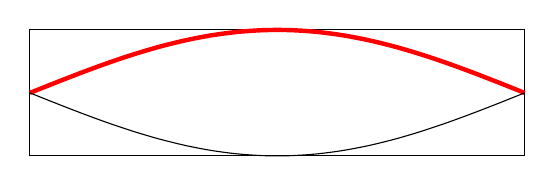
\begin{tikzpicture}[scale=2,yscale=.4]
      \draw(0,-1) rectangle(pi,1);
      \draw[smooth,samples=20,domain=0:pi,red,ultra thick]
      plot({\x},{sin(180/pi*\x)});
      \draw[smooth,samples=20,domain=0:pi] plot({\x},{-1*sin(180/pi*\x)});
    \end{tikzpicture}
    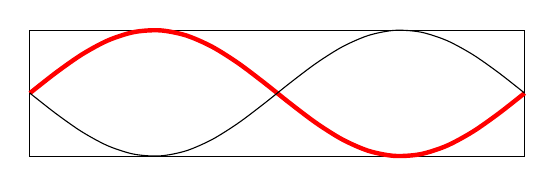
\begin{tikzpicture}[scale=2,yscale=.4]
      \draw(0,-1) rectangle(pi,1);
      \draw[smooth,samples=20,domain=0:pi,red,ultra thick]
      plot({\x},{sin(360/pi*\x)});
      \draw[smooth,samples=20,domain=0:pi] plot({\x},{-1*sin(360/pi*\x)});
    \end{tikzpicture}\\
    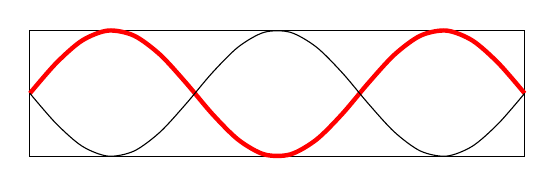
\begin{tikzpicture}[scale=2,yscale=.4]
      \draw(0,-1) rectangle(pi,1);
      \draw[smooth,samples=20,domain=0:pi,red,ultra thick]
      plot({\x},{sin(540/pi*\x)});
      \draw[smooth,samples=20,domain=0:pi] plot({\x},{-1*sin(540/pi*\x)});
    \end{tikzpicture}
    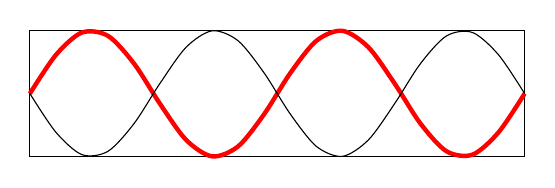
\begin{tikzpicture}[scale=2,yscale=.4]
      \draw(0,-1) rectangle(pi,1);
      \draw[smooth,samples=20,domain=0:pi,red,ultra thick]
      plot({\x},{sin(720/pi*\x)});
      \draw[smooth,samples=20,domain=0:pi] plot({\x},{-1*sin(720/pi*\x)});
    \end{tikzpicture}
  \end{center}
  The air molecules at the end of the pipe cannot vibrate along the direction of
  wave motion, therefore they have to be nodes. This pattern is identical to
  that of the vibrating string.
\end{frame}


\begin{frame}{Standing Waves in Closed Pipes}
  Like strings, pipes that are \emph{closed at both ends} have resonance
  frequencies that are whole-number multiple of the fundamental frequency $f_1$:
  
  \eq{-.2in}{
    \boxed{f_n=nf_1=n\frac{v_s}{2L}}\quad n=1,2,3,\ldots
  }
  
  And the wavelengths corresponding to the resonance frequencies are:

  \eq{-.2in}{
    \boxed{\lambda=\frac{2L}n}\quad n=1,2,3,\ldots
  }

  The difference between a closed pipe and a string is that the wave speed is
  now the speed of sound $v_s$ inside the pipe.
\end{frame}



\begin{frame}{Standing Waves in Open Pipes}
  Many types of organ pipes, as well as the flute, can be modelled as pipes
  that are open on both ends. The standing-wave patterns for open pipes are
  similar to strings and closed pipes, but with nodes and anti-nodes reversed:
  \begin{center}
    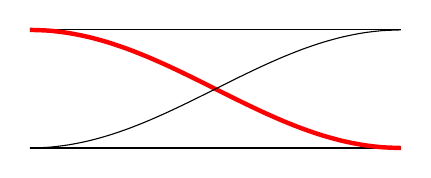
\begin{tikzpicture}[scale=1.5]
      \draw(0,-.5)--(pi,-.5);
      \draw(0,0.5)--(pi,0.5);
      \draw[smooth,samples=20,domain=0:pi,red,ultra thick]
         plot({\x},{0.5*sin(180/pi*\x+90)});
      \draw[smooth,samples=20,domain=0:pi]
        plot({\x},{-.5*sin(180/pi*\x+90)});
    \end{tikzpicture}
    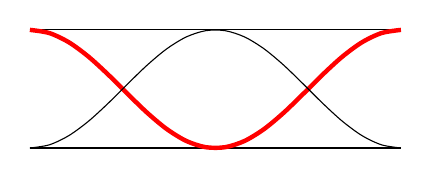
\begin{tikzpicture}[scale=1.5]
      \draw(0,-.5)--(pi,-.5);
      \draw(0,0.5)--(pi,0.5);
      \draw[smooth,samples=20,domain=0:pi,red,ultra thick]
        plot({\x},{0.5*sin(360/pi*\x+90)});
      \draw[smooth,samples=20,domain=0:pi]
        plot({\x},{-.5*sin(360/pi*\x+90)});
    \end{tikzpicture}\\
    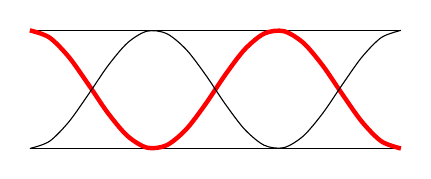
\begin{tikzpicture}[scale=1.5]
      \draw(0,-.5)--(pi,-.5);
      \draw(0,0.5)--(pi,0.5);
      \draw[smooth,samples=20,domain=0:pi,red,ultra thick]
      plot({\x},{0.5*sin(540/pi*\x+90)});
      \draw[smooth,samples=20,domain=0:pi]
      plot({\x},{-.5*sin(540/pi*\x+90)});
    \end{tikzpicture}
    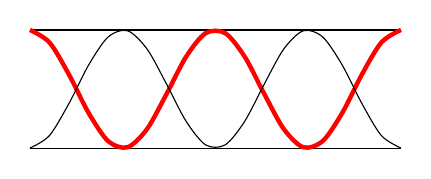
\begin{tikzpicture}[scale=1.5]
      \draw(0,-.5)--(pi,-.5);
      \draw(0,0.5)--(pi,0.5);
      \draw[smooth,samples=20,domain=0:pi,red,ultra thick]
      plot({\x},{0.5*sin(720/pi*\x+90)});
      \draw[smooth,samples=20,domain=0:pi]
      plot({\x},{-.5*sin(720/pi*\x+90)});
    \end{tikzpicture}
  \end{center}
  The air molecules at the ends of the pipe have maximum vibrations, and are
  anti-nodes in the standing wave.
%  \begin{columns}
%    \column{.5\textwidth}
%    First resonance at $\lambda=2L$
%    \begin{displaymath}
%      f_1=\frac{v_s}{\lambda}=\frac{v_s}{2L}
%    \end{displaymath}
%    \column{.5\textwidth}
%    Second resonance at $\lambda=L$
%    \begin{displaymath}
%      f_2=\frac{v_s}{\lambda}=\frac{v_s}{L}=2f_1
%    \end{displaymath}
%  \end{columns}
\end{frame}



\begin{frame}{Standing Waves in Open Pipes}
  Not surprisingly, like strings and closed pipes, open pipes have resonance
  frequencies that are whole-number multiple of the fundamental frequency $f_1$:
  
  \eq{-.2in}{
    \boxed{f_n=nf_1=n\frac{v_s}{2L}}\quad n=1,2,3,\ldots
  }
  
  And the wavelengths corresponding to the resonance frequencies are also
  identical to that of the closed pipes.

  \eq{-.2in}{
    \boxed{\lambda=\frac{2L}n}\quad n=1,2,3,\ldots
  }
  Strings, closed pipes and open pipes are all said to have
  ``full set of harmonics'' because every harmonic frequency is also a
  resonance frequency.
\end{frame}


\begin{frame}{Standing Waves in Semi-Open Pipes}
  However, most organ pipes, woodwind and brass instruments are in fact
  modelled as pipes that are \emph{closed at one end and open at the other}
  \begin{center}
    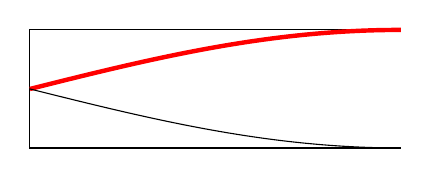
\begin{tikzpicture}[scale=1.5]
      \draw(pi,-.5)--(0,-.5)--(0,.5)--(pi,.5);
      \draw[smooth,samples=20,domain=0:pi,red,ultra thick]
         plot({\x},{0.5*sin(90/pi*\x)});
      \draw[smooth,samples=20,domain=0:pi]
        plot({\x},{-.5*sin(90/pi*\x)});
    \end{tikzpicture}
    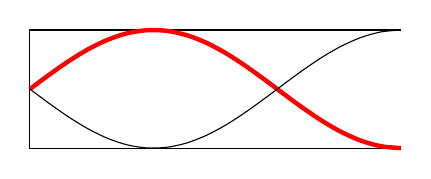
\begin{tikzpicture}[scale=1.5]
      \draw(pi,-.5)--(0,-.5)--(0,.5)--(pi,.5);
      \draw[smooth,samples=20,domain=0:pi,red,ultra thick]
        plot({\x},{0.5*sin(270/pi*\x)});
      \draw[smooth,samples=20,domain=0:pi]
        plot({\x},{-.5*sin(270/pi*\x)});
    \end{tikzpicture}\\
    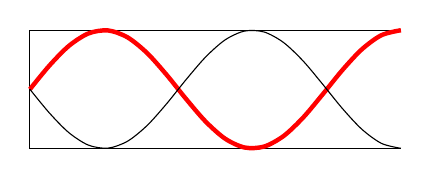
\begin{tikzpicture}[scale=1.5]
      \draw(pi,-.5)--(0,-.5)--(0,.5)--(pi,.5);
      \draw[smooth,samples=20,domain=0:pi,red,ultra thick]
      plot({\x},{0.5*sin(450/pi*\x)});
      \draw[smooth,samples=20,domain=0:pi]
      plot({\x},{-.5*sin(450/pi*\x)});
    \end{tikzpicture}
    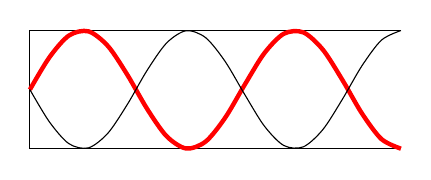
\begin{tikzpicture}[scale=1.5]
      \draw(pi,-.5)--(0,-.5)--(0,.5)--(pi,.5);
      \draw[smooth,samples=20,domain=0:pi,red,ultra thick]
      plot({\x},{0.5*sin(630/pi*\x)});
      \draw[smooth,samples=20,domain=0:pi]
      plot({\x},{-.5*sin(630/pi*\x)});
    \end{tikzpicture}
  \end{center}
  The closed end is a node (like in the closed pipes), while the open end is
  an anti-node (like in the open pipes).
\end{frame}

\begin{frame}
  \frametitle{Standing Waves in Semi-Open Pipes}
  Again starting with the fundamental frequency (lowest frequency where a
  standing wave can form inside the pipe). This occurs at $\lambda=4L$:

  \vspace{-.1in}
  \begin{center}
    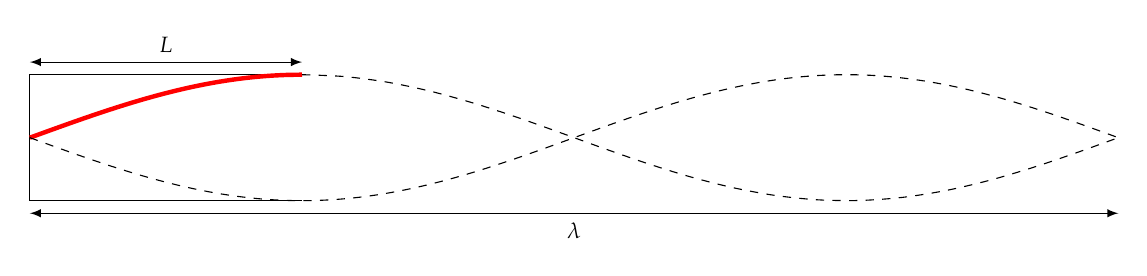
\begin{tikzpicture}[xscale=1.1,yscale=.8]
      \draw(pi,-1)--(0,-1)--(0,1)--(pi,1);
      \draw[smooth,samples=20,domain=0:pi,red,ultra thick]
      plot({\x},{sin(90/pi*\x)});
      \draw[smooth,samples=20,domain=pi:4*pi,dashed]
      plot({\x},{sin(90/pi*\x)});
      \draw[smooth,samples=80,domain=0:4*pi,dashed]
      plot({\x},{-1*sin(90/pi*\x)});
      \draw[<->](0,1.2)--(pi,1.2)
      node[midway,above]{\footnotesize $L$};
      \draw[<->](0,-1.2)--(4*pi,-1.2)
      node[midway,below]{\footnotesize $\lambda$};
    \end{tikzpicture}
  \end{center}
  
  Fundamental frequency $f_1$ is lower than the open-pipe and closed-pipe of
  the same length by a factor of 2:

  \eq{-.2in}{
    \boxed{f_1=\frac{v_s}{\lambda}=\frac{v_s}{4L}}
  }
\end{frame}



\begin{frame}{Standing Waves in Semi-Open Pipes}
  Likewise, second resonance can be found at $\displaystyle\lambda=\frac43L$:
  \begin{columns}
    \column{.45\textwidth}
    \centering
    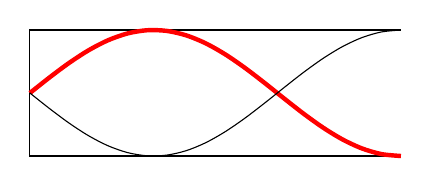
\begin{tikzpicture}[xscale=1.5,yscale=.8]
      \draw(pi,-1)--(0,-1)--(0,1)--(pi,1);
      \draw[smooth,samples=20,domain=0:pi,red,ultra thick]
      plot({\x},{sin(270/pi*\x)});
      \draw[smooth,samples=20,domain=0:pi] plot({\x},{-1*sin(270/pi*\x)});
    \end{tikzpicture}
    
    \column{.55\textwidth}

    \eq{-.4in}{
      f_{\text{res},2}=\frac{v_s}{\lambda}=\frac{3v_s}{4L}=3f_1
    }
  \end{columns}
  And then, third resonance at $\displaystyle\lambda=\frac45L$:
  \begin{columns}

    \column{.45\textwidth}
    \centering
    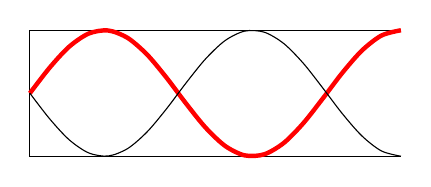
\begin{tikzpicture}[xscale=1.5,yscale=.8]
      \draw(pi,-1)--(0,-1)--(0,1)--(pi,1);
      \draw[smooth,samples=20,domain=0:pi,red,ultra thick]
      plot({\x},{sin(450/pi*\x)});
      \draw[smooth,samples=20,domain=0:pi] plot({\x},{-1*sin(450/pi*\x)});
    \end{tikzpicture}

    \column{.55\textwidth}
    \eq{-.2in}{
      f_{\text{res},3}=\frac{v_s}{\lambda}=\frac{5v_s}{4L}=5f_1
    }
  \end{columns}
\end{frame}



\begin{frame}{Standing Waves in Semi-Open Pipes}
  Only \textbf{odd-number multiples} of the fundamental frequency are resonance
  frequencies in a semi-open pipe.  We say that semi-open pipes have an
  \emph{odd} set of harmonics.

  \eq{-.25in}{
    \boxed{f_n = (2n-1)f_1=\frac{(2n-1)v_s}{4L}}\quad n=1,2,3,\ldots
  }
  
  Because fundamental frequency $f_1$ is lower than the open-pipe configuration
  by a factor of 2 for the same length $L$, it has advantages when designing an
  organ pipe.
\end{frame}


%\begin{frame}
%  \frametitle{Resonance \emph{Length} in a Semi-Open Pipe}
%  \begin{itemize}
%  \item Now that we have looked at resonance \emph{frequencies}, we'll look
%    at resonance \emph{lengths}
%  \item We produce a single frequency in the pipe, and vary the length of the
%    pipe until we have resonance
%  \end{itemize}
%\end{frame}
%
%\begin{frame}
%  \frametitle{Resonance Length in a Semi-Open Pipe}
%  Let's submerge a part of this pipe in water\ldots
%  \begin{center}
%    \pic{.7}{res-length-closed}
%  \end{center}
%\end{frame}
%
%\begin{frame}
%  \frametitle{Resonance Length in a Semi-Open Pipe}
%  The resonance lengths are \textbf{odd whole-number multiples} of the first
%  resonance length $L_1$: %($\displaystyle\frac{\lambda}{4}$):
%  
%  \eq{-.2in}{
%    \boxed{L_{\text{res},n} = (2n-1)L_1}
%    \quad\text{\normalsize where}\quad
%    \boxed{L_1 = \frac{\lambda}{4}}
%  }
%\end{frame}
%
%
%
%\begin{frame}
%  \frametitle{Resonance in an Open Pipe}
%  We can also repeat this with pipes that are open on both ends.
%  \begin{center}
%    \pic{.75}{res-length-open}
%  \end{center}
%\end{frame}
%
%
%
%\begin{frame}
%  \frametitle{Resonance in an Open Pipe}
%  Resonance lengths of an open pipe are \textbf{whole-number multiples} of the
%  first resonance length $L_1$:
%
%  \eq{-.25in}{
%    \boxed{L_{\text{res},n}=nL_1}
%    \quad\text{\normalsize (open pipe)}
%  }
%  
%  \vspace{-.1in}where first resonance length is given by:
%  
%  \eq{-.2in}{
%    \boxed{L_1=\frac{\lambda}{2}}
%  }
%  
%  Be careful! This equation looks a lot like the resonance frequency equation!
%\end{frame}

\begin{frame}{Your Piano is \textbf{Always} Out of Tune!}
  \begin{itemize}
  \item The concept of harmonic frequencies is the reason why some musical
    instruments will never play well in harmony (e.g.\ pianos, modern organs).
  \item \textbf{Example:} Find all the harmonics of a fundamental frequency of
    \SI{110}\hertz and then compare them to the values on the table.
  \end{itemize}
  \begin{center}
    \pic{.6}{fundamental_freqs}
  \end{center}
\end{frame}
\end{document}
